% lint-skip: 未完成ステータス（figure/table caption 未対応，人手チェック時に解消予定）
\documentclass[../../main.tex]{subfiles}
\begin{document}

\begin{flushright}
  \footnotesize\textit{【自動文字起こし・要確認】}
\end{flushright}

\noindent
{\bf [解答]}

\begin{enumerate}
  \item[(1)] 右のグラフから
    \begin{itemize}
      \item $l < 0$ の時, $x \leqq l$ をみたす $x$ に対して $x^2 > 0 > l$ となり, $S$ には属さない.
      \item $l > 1$ の時, $x = l$ での題意の成立が必要だが,
        \[
          l^2 - l = l(l-1) > 0
        \]
        となって $l^2 < l$ に矛盾.
    \end{itemize}
    よって, $0 \leqq l \leqq 1$ である.

    \begin{figure}[htb]
      \centering
      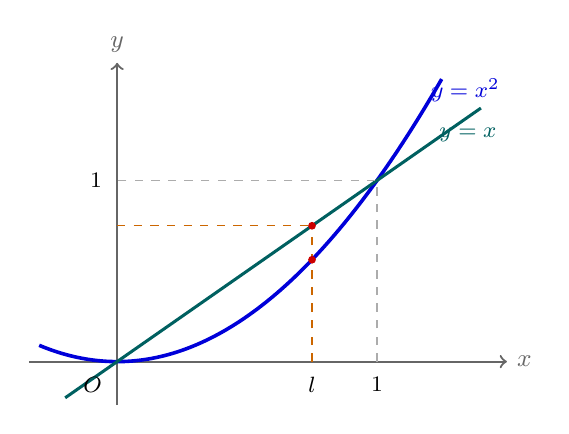
\begin{tikzpicture}[x=3.3cm, y=2.3cm,
        every node/.style={font=\small}]
        % l=3/4 illustrates the required range 0<l<1.
        \draw[->, thick, gray!80!black] (-0.34,0)--(1.5,0)
        node[right] {$x$};
        \draw[->, thick, gray!80!black] (0,-0.24)--(0,1.65)
        node[above] {$y$};
        \draw[line width=1.3pt, blue!85!black,
        domain=-0.3:1.25, samples=80, smooth]
        plot (\x,{\x*\x});
        \draw[line width=1.1pt, teal!75!black] (-0.2,-0.2)
        -- (1.4,1.4);
        \draw[dashed, gray!65] (1,0)--(1,1)--(0,1);
        \draw[dashed, orange!80!black] (0.75,0)--(0.75,0.75)
        (0,0.75)--(0.75,0.75);
        \fill[red!80!black] (0.75,0.5625) circle(1.4pt);
        \fill[red!80!black] (0.75,0.75) circle(1.4pt);
        \node[below left=2pt, font=\footnotesize] at (0,0) {$O$};
        \node[below=2pt, font=\footnotesize] at (0.75,0) {$l$};
        \node[below=2pt, font=\footnotesize] at (1,0) {$1$};
        \node[left=2pt, font=\footnotesize] at (0,1) {$1$};
        \node[blue!85!black, font=\footnotesize] at (1.34,1.5)
        {$y=x^2$};
        \node[teal!75!black, font=\footnotesize] at (1.35,1.25)
        {$y=x$};
      \end{tikzpicture}
      \caption{$y=x^2$ と $y=x$ の比較（図は $l=3/4$）}
      \label{fig:1968_3_basic_comparison}
    \end{figure}

  \item[(2)]
    \begin{itemize}
      \item $0 < m < 1$ とすると, $x = m$ での題意の成立が必要だが ($m \leqq l \leqq 1$ だから)
        \[
          m^2 - m = m(m-1) < 0 \implies m^2 < m
        \]
        となり矛盾.
      \item $1 < m$ とすると, $1 < m \leqq l$ となり, (1) から $0 \leqq l \leqq 1$ であることに反する.
    \end{itemize}
    以上から $m \leqq 0$ または $m = 1$ である.

  \item[(3)] $m = 1$ の時, $0 \leqq l \leqq 1$ と $1 \leqq l$ から $l = 1$ であり,
    \[
      S = \{1\}
    \]

  \item[(4)] $m < 0$ の時, $m \leqq x \leqq l$ の全ての $x$ で $m \leqq x^2 \leqq l$ となるような $m$ を求める.
    $x^2 = l \iff x = \pm \sqrt{l}$ から, グラフは右のようになり, 条件は
    \[
      -\sqrt{l} \leqq m \leqq 0
    \]
    である.

    \begin{figure}[htb]
      \centering
      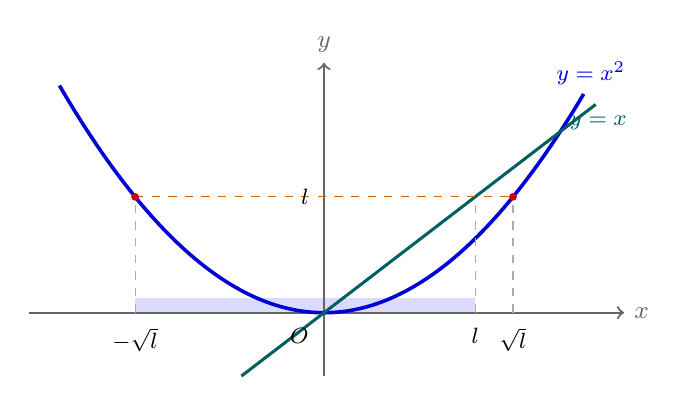
\begin{tikzpicture}[x=3cm, y=2.3cm,
        every node/.style={font=\small}]
        % l=16/25, hence sqrt(l)=4/5 and -sqrt(l)=-4/5.
        \fill[blue!14] (-0.8,0) rectangle (0.64,0.08);
        \draw[->, thick, gray!80!black] (-1.25,0)--(1.27,0)
        node[right] {$x$};
        \draw[->, thick, gray!80!black] (0,-0.35)--(0,1.38)
        node[above] {$y$};
        \draw[line width=1.3pt, blue!85!black,
        domain=-1.12:1.1, samples=90, smooth]
        plot (\x,{\x*\x});
        \draw[line width=1.1pt, teal!75!black] (-0.35,-0.35)
        -- (1.15,1.15);
        \draw[dashed, orange!80!black] (-0.8,0.64)
        -- (0.8,0.64);
        \draw[dashed, gray!65] (-0.8,0)--(-0.8,0.64)
        (0.64,0)--(0.64,0.64)
        (0.8,0)--(0.8,0.64);
        \fill[red!80!black] (-0.8,0.64) circle(1.4pt);
        \fill[red!80!black] (0.8,0.64) circle(1.4pt);
        \node[below left=2pt, font=\footnotesize] at (0,0) {$O$};
        \node[below=2pt, font=\footnotesize] at (-0.8,0)
        {$-\sqrt l$};
        \node[below=2pt, font=\footnotesize] at (0.64,0) {$l$};
        \node[below=2pt, font=\footnotesize] at (0.8,0)
        {$\sqrt l$};
        \node[left=2pt, font=\footnotesize] at (0,0.64) {$l$};
        \node[blue!85!black, font=\footnotesize] at (1.13,1.32)
        {$y=x^2$};
        \node[teal!75!black, font=\footnotesize] at (1.16,1.05)
        {$y=x$};
      \end{tikzpicture}
      \caption{$x^2\le l$ となる区間と $m\ge-\sqrt l$（図は $l=16/25$）}
      \label{fig:1968_3_negative_lower_bound}
    \end{figure}
\end{enumerate}

\newpage

\end{document}
